%%%%%%%%%%%%%%%%%%%%% Reporte %%%%%%%%%%%%%%%%%%%%%
\documentclass[12pt, a4paper]{report}
\usepackage[spanish]{babel}
\usepackage[utf8]{inputenc}
%%%%%%%%%%%%%%%%%%%%% Paquetes %%%%%%%%%%%%%%%%%%%}		
\usepackage{geometry}
\usepackage{graphicx}
\usepackage{amssymb,amsmath,amsthm,amstext,amsfonts}
\usepackage{color}


\setlength{\parindent}{0pt}

\graphicspath{ {Img/} }

% Colors for the hyperref package
\definecolor{urlcolor}{rgb}{0,.145,.698}
\definecolor{linkcolor}{rgb}{.71,0.21,0.01}
\definecolor{citecolor}{rgb}{.12,.54,.11}

%%%%%%%%%%%% NEW THEOREM %%%%%%%%%%%%%%%%%
\providecommand{\abs}[1]{\lvert#1\rvert}
\newtheorem{definition}{Definición}
\newtheorem{proposition}{Proposición}
\newtheorem{remark}{Observación}
\newtheorem{notation}{Notación}
\newtheorem{lemma}{Lema}
\newtheorem{theorem}{Teorema}
\newtheorem{example}{Ejemplo}
%%%%%%%%%%%%%%%%%%%%%%%%%%%%%%%%%%%%%%%%%%%%%%%%%

\title{Tesis de posgrado.}
\author{Eduardo Ortiz Romero}

%%%%%%%%%%%%%%%%%%%%%%%%%%%%%%%%%%%%%%%%%%%%%%%

\begin{document}
\maketitle
\tableofcontents

\chapter{Introducción}

\begin{figure}[h]
	\centering
	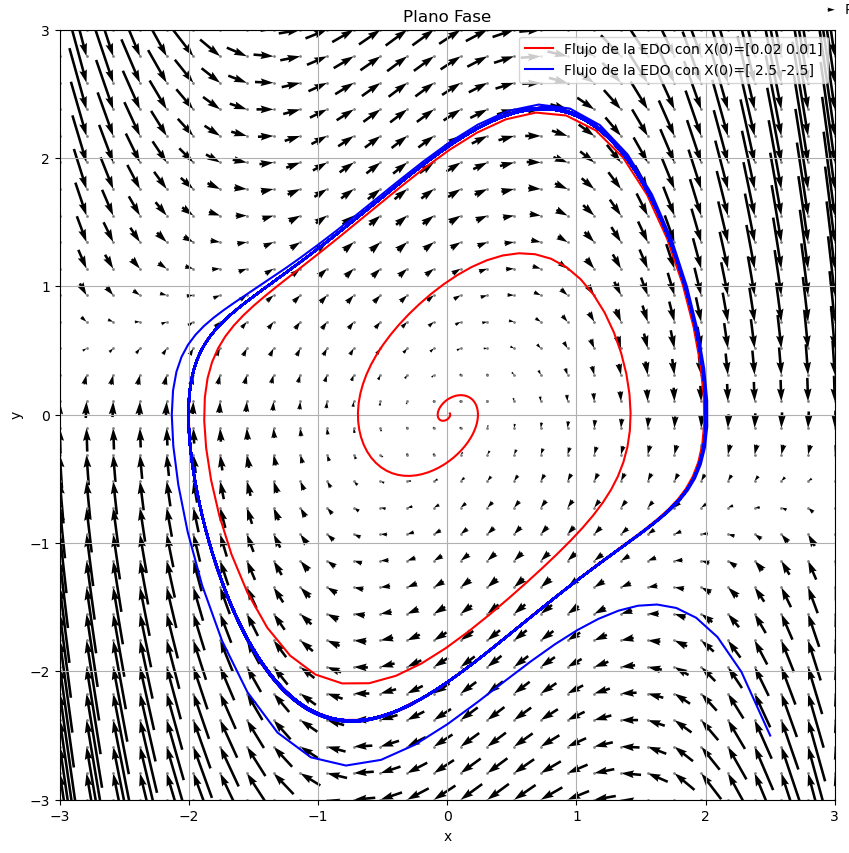
\includegraphics[width=8cm]{portada.png}
\end{figure}

\section{Problema 16 de Hilbert}
En 1900, el matemático alemán David Hilbert presentó una lista de 23 problemas abiertos en el Congreso Internacional de Matemáticos en París. Estos problemas de diversas áreas de las matemáticas, se convirtieron en una guía fundamental para la investigación matemática del siglo XX y, en muchos casos, aún siguen desafiando a la comunidad científica.\\

El \textbf{problema 16 de Hilbert}  forma parte de esta lista y está dividido en dos partes principales. Ambas se centran en el análisis geométrico y topológico de curvas algebraicas y sistemas dinámicos polinomiales en el plano:

\begin{enumerate}
	\item \textbf{Primera parte:} Clasificar las disposiciones topológicas posibles de las curvas algebraicas planas reales de grado $n$. Este problema está relacionado con la geometría algebraica real y la topología.
	\item \textbf{Segunda parte:} Estudiar los sistemas dinámicos definidos por campos vectoriales polinomiales en el plano, y en particular, determinar el número máximo y la disposición de los ciclos límite que estos sistemas pueden tener.
\end{enumerate}

La segunda parte del problema 16 de Hilbert aborda una cuestión fundamental en la teoría de sistemas dinámicos: la existencia, finitud y disposición de ciclos límite en sistemas de ecuaciones diferenciales polinomiales. Un ciclo límite es una órbita cerrada aislada en el espacio de fases, alrededor de la cual las trayectorias vecinas convergen o divergen en espiral hacia adentro o hacia afuera.\\

Consideremos el sistema de ecuaciones  en el plano polinomial de grado $n$:

\begin{equation}
	x'=P\left(x,y\right)\text{, }\text{  }y'=Q\left(x,y\right)
\end{equation}
donde $P\left(x,y\right)$ y $Q\left(x,y\right)$ son polinomios de grado a lo más $n$. El problema consiste en responder las siguientes preguntas:
\begin{enumerate}
	\item ¿Cuántos ciclos límite puede tener un sistema polinómico de grado $n$?
	\item ¿Cómo están distribuidos estos ciclos límite en el plano?
\end{enumerate}

¿Sencillo? pues no, la respuesta sigue siendo desconocida para $n>1$, sin embargo tenemos algunos resultados significativos como la conjetura de Dulac, que establece que para cualquier n, el número de ciclos límite de un sistema polinómico de grado $n$ es finito, sin embargo esto es una conjetura y aún no se ha probado. El teorema de Poincaré- Bendixón por otro lado establece las condiciones suficientes para la existencia de ciclos límite en sistemas planares. Este teorema será central en el análisis de esta tésis.

\section{Importancia de los ciclos límite}

Los sistemas dinámicos ofrecen la posibilidad de explorar comportamientos oscilatorios que son inherentes a muchos procesos biológicos, químicos y físicos. A continuación, se presentan varios ejemplos donde los ciclos límite desempeñan un papel central.

\begin{itemize}
	\item \textbf{Oscilador de Van der Pol}\\
	
	El oscilador de Van der Pol es un ejemplo clásico de un sistema no lineal que exhibe ciclos límite. Originalmente desarrollado para modelar circuitos eléctricos con tubos de vacío, este sistema también describe fenómenos auto-oscilatorios en ingeniería y biología.
	\begin{equation}
		x''-\mu \left(1-x^2\right)x'+x=0
	\end{equation}
	donde $\mu$ es el coeficiente de amortiguamiento.  A medida que $\mu$ aumenta, el sistema muestra un ciclo límite estable que corresponde a una oscilación sostenida. Este comportamiento es crucial para entender dispositivos electrónicos oscilatorios y ciertos ritmos biológicos.
	\item \textbf{Ecuación de Rayleigh}\\
	
	La ecuación de Rayleigh modela el comportamiento de ciertos sistemas mecánicos y fluidos sometidos a fuerzas periódicas. Es similar al oscilador de Van der Pol.
	\begin{equation}
		x''+x=\epsilon\left(1-x'^2\right)x'
	\end{equation}
	donde $\epsilon$ controla la intensidad de la fuerza. Los ciclos límite en este modelo describen el fenómeno de resonancia mecánica y son fundamentales para el diseño de sistemas que requieren estabilidad en las oscilaciones, como los amortiguadores en vehículos.
	\item \textbf{Modelo de FitzHugh-Nagumo}\\
	
	Este modelo es una simplificación del modelo de Hodgkin-Huxley y se utiliza para describir la activación y desactivación de las neuronas. 
	\begin{equation}
		\begin{matrix}
			v'=v-\frac{v^3}{3}-w+I\\
			w'=\epsilon\left(v+a-bw\right)
		\end{matrix}
	\end{equation}
	donde $v$ representa el potencial de membrana, $w$ es una variable de recuperación, e $I$ es un término de corriente externa. Los ciclos límite en este sistema modelan los potenciales de acción neuronal, esenciales para entender el procesamiento de la información en el cerebro.\\
\newpage

	\item \textbf{Reacciones Químicas Oscilatorias}\\
	
	Un ejemplo destacado es la reacción de Belousov-Zhabotinsky, que es un tipo de reacción química que muestra oscilaciones temporales en la concentración de sus reactivos. Aunque su modelado exacto requiere ecuaciones más complejas, sistemas simplificados que muestran ciclos límite pueden ayudar a comprender la dinámica subyacente de estas reacciones oscilatorias.
\end{itemize}
Más adelante vamos desarrollar estos modelos a profundidad.
\newpage

\chapter{Preliminares}

\section{Coordenadas polares}

Consideremos las variables $(x,y)\in\mathbb{R}^2$, las cuales están parametrizadas en términos del tiempo $t$, es decir, $x=x(t)$ & $y=y(t)$ con parámetro $t\geq0$. Definimos el cambio de coordenadas cartesianas $(x,y)$
a coordenadas polares $(r,\theta)$  mediante las relaciones:
\begin{equation}\label{eq: xpolar}
	x=r\cos(\theta)
\end{equation}

\begin{equation}\label{eq: ypolar}
	y=r\sin(\theta)
\end{equation}

donde $r=r(t)$ & $\theta=\theta(t)$ también están parametrizadas en términos de $t$.\\

Estas ecuaciones nos llevan a las siguientes identidades:

\begin{equation}\label{eq: r2}
	r^2=x^2+y^2\\
\end{equation}

\begin{equation}\label{eq: theta}
	\theta=\arctan{(\frac{y}{x})}
\end{equation}

en este caso restringimos $\theta\in\left[-\frac{\pi}{2},\frac{\pi}{2}\right]$.\\

Derivamos las ecuaciones \eqref{eq: r2} y \eqref{eq: theta} respecto a $t$, obtenemos las relaciones dinámicas en coordenadas polares:

\begin{equation}\label{eq: drcart}
	rr'=xx'+yy'
\end{equation}

\begin{equation}\label{eq: dthetacart}
	r^2\theta'=xy'-yx'
\end{equation}

\newpage

\section{Teoría de perturbaciones}

Definimos un \textbf{problema perturbado} como una ecuación 

\begin{equation}\label{eq: problemaPerturbado}
	P^\epsilon\left(x\right)=0
\end{equation}

que incluye un parámetro pequeño $\epsilon$ con $0<\epsilon<1$, el cual que representa la perturbación.\\

El objetivo es encontrar soluciones aproximadas $x=x\left(\epsilon\right)$ en función de este parámetro y estudiar su comportamiento cuando $\epsilon\to0$\\

Para estudiar el comportamiento asintótico de las soluciones vamos a introducir el concepto de función de orden.

\begin{definition}[Función de orden]
	Se dice que una función $\delta=\delta\left(\epsilon\right)$ es de orden si cumple las siguientes condiciones:
	\begin{enumerate}
		\item Es continua en una vecindad de $\epsilon=0$.
		\item Tiene signo definido en esa vecindad (es decir, $\delta(\epsilon)>0$ o $\delta(\epsilon)<0$ para $0<\epsilon<\epsilon_0$ con $\epsilon_0>0$).
		\item Esiste el límite:
		$$\large\lim_{\epsilon\to0}\delta\left(\epsilon\right)$$
	\end{enumerate}
\end{definition}

\begin{definition}
	Sean $\delta_1\left(\epsilon\right)$ y $\delta_2\left(\epsilon\right)$ funciones de orden. Decimos que: 
	\begin{enumerate}
		\item $\delta_1\left(\epsilon\right)=O\left(\delta_2\left(\epsilon\right)\right)$ si existe $k\in\mathbb{R}^+$ y un $\epsilon_0>0$ tales que:
		\begin{equation}\label{eq: Big-O}
			|\delta_1\left(\epsilon\right)|\leq k|\delta_2\left(\epsilon\right)|
		\end{equation}
		para todo $0<\epsilon<\epsilon_0$.\\

		Esta definición describe una cota superior en el crecimiento de la función $\delta_1\left(\epsilon\right)$ en términos de $\delta_2\left(\epsilon\right)$ cuando $\epsilon\to0$. Es decir, $\delta_2(\epsilon)$ actúa como una cota superior para $\delta_1(\epsilon)$.\\
		\item $\delta_1\left(\epsilon\right)=o(\delta_2\left(\epsilon\right))$ si:
		\begin{equation}\label{eq: small-o}
			\large\lim_{\epsilon\to0}\frac{\delta_1\left(\epsilon\right)}{\delta_2\left(\epsilon\right)}=0
		\end{equation}
		Esta definición indica que $\delta_1\left(\epsilon\right)$ es asintóticamente insignificante en comparación con $\delta_2\left(\epsilon\right)$ cuando $\epsilon\to0$; es decir, $\delta_2(\epsilon)$ crece (o decrece) más rápido que $\delta_1(\epsilon)$\\
	\end{enumerate}
\end{definition} 

Consideremos las funciones $\delta_1\left(\epsilon\right)=\ln\left(1+\epsilon\right)$ y $\delta_2\left(\epsilon\right)=\epsilon$.\\

La serie de Taylor de $\ln\left(1+\epsilon\right)$ alrededor de $\epsilon=0$ es:

$$\ln\left(1+\epsilon\right)=\epsilon-\frac{\epsilon^2}{2}+\frac{\epsilon^3}{3}-\dots$$

evaluamos el límite:

$$\large\lim_{\epsilon\to0}\frac{\delta_1\left(\epsilon\right)}{\delta_2\leftp|(\epsilon\right)}=\lim_{\epsilon\to0}\frac{\epsilon-\frac{\epsilon^2}{2}+\frac{\epsilon^3}{3}-\dots}{\epsilon}=\lim_{\epsilon\to0}\left(1-\frac{\epsilon}{2}+\frac{\epsilon^2}{3}-\dots\right)=1.$$

El límite es distinto de cero, por lo que $\ln\left(1+\epsilon\right)$ no es $o\left(\epsilon\right)$. Sin embargo, dado que el límite es finito y positivo, concluimos que $\ln\left(1+\epsilon\right)=O\left(\epsilon\right)$.\\

Veamos algunos ejemplos más para comprender mejor estas definiciones.

\subsection*{Ejemplos para \( O\left( \delta_2(\epsilon) \right) \)}

\subsubsection*{Ejemplo 1}

Sea \(\delta_1(\epsilon) = \sin(\epsilon)\) y \(\delta_2(\epsilon) = \epsilon\).

Sabemos que para \(\epsilon \to 0\):

\[
\sin(\epsilon) = \epsilon - \frac{\epsilon^3}{6} + \frac{\epsilon^5}{120} - \dots
\]

Calculamos el límite:

\[
\lim_{\epsilon \to 0} \frac{\sin(\epsilon)}{\epsilon} = \lim_{\epsilon \to 0} \left(1 - \frac{\epsilon^2}{6} + \frac{\epsilon^4}{120} - \dots \right) = 1.
\]

El límite es finito y positivo, por lo que \(\sin(\epsilon) = O\left( \epsilon \right)\).

\subsubsection*{Ejemplo 2}

Sea \(\delta_1(\epsilon) = e^\epsilon - 1\) y \(\delta_2(\epsilon) = \epsilon\).

La serie de Taylor de \(e^\epsilon\) es:

\[
e^\epsilon = 1 + \epsilon + \frac{\epsilon^2}{2} + \frac{\epsilon^3}{6} + \dots
\]

Entonces:

\[
e^\epsilon - 1 = \epsilon + \frac{\epsilon^2}{2} + \frac{\epsilon^3}{6} + \dots
\]

Calculamos el límite:

\[
\lim_{\epsilon \to 0} \frac{e^\epsilon - 1}{\epsilon} = \lim_{\epsilon \to 0} \left(1 + \frac{\epsilon}{2} + \frac{\epsilon^2}{6} + \dots \right) = 1.
\]

Por lo tanto, \(e^\epsilon - 1 = O\left( \epsilon \right)\).

\subsection*{Ejemplos para \( o\left( \delta_2(\epsilon) \right) \)}

\subsubsection*{Ejemplo 3}

Sea \(\delta_1(\epsilon) = \epsilon^2\) y \(\delta_2(\epsilon) = \epsilon\).

Calculamos el límite:

\[
\lim_{\epsilon \to 0} \frac{\epsilon^2}{\epsilon} = \lim_{\epsilon \to 0} \epsilon = 0.
\]

Entonces, \(\epsilon^2 = o\left( \epsilon \right)\), lo que significa que \(\epsilon^2\) es insignificante en comparación con \(\epsilon\) cuando \(\epsilon \to 0\).

\subsubsection*{Ejemplo 4}

Sea \(\delta_1(\epsilon) = \epsilon \ln(\epsilon)\) y \(\delta_2(\epsilon) = \epsilon\).

Para \(\epsilon \to 0^+\), \(\ln(\epsilon) \to -\infty\), por lo que \(\epsilon \ln(\epsilon) \to 0^-\).

Calculamos el límite:

\[
\lim_{\epsilon \to 0^+} \frac{\epsilon \ln(\epsilon)}{\epsilon} = \lim_{\epsilon \to 0^+} \ln(\epsilon) = -\infty.
\]

Aunque el límite es infinito negativo, observamos que \(\epsilon \ln(\epsilon)\) tiende a cero más lentamente que \(\epsilon\). Por lo tanto, \(\epsilon \ln(\epsilon) = o(1)\), pero no es \(o\left( \epsilon \right)\) ni \(O\left( \epsilon \right)\).

\subsubsection*{Ejemplo 5}

Sea \(\delta_1(\epsilon) = e^{-1/\epsilon}\) y \(\delta_2(\epsilon) = \epsilon^n\) para cualquier \(n > 0\).

Cuando \(\epsilon \to 0^+\):

\[
e^{-1/\epsilon} \to e^{-\infty} = 0,
\]

y

\[
\lim_{\epsilon \to 0^+} \frac{e^{-1/\epsilon}}{\epsilon^n} = 0,
\]

ya que \(e^{-1/\epsilon}\) decrece más rápidamente que cualquier potencia de \(\epsilon\). Por lo tanto, \(e^{-1/\epsilon} = o\left( \epsilon^n \right)\).

\subsubsection*{Ejemplo 6}

Sea \(\delta_1(\epsilon) = \epsilon^n\) y \(\delta_2(\epsilon) = e^{-1/\epsilon}\) para cualquier \(n > 0\).

Calculamos:

\[
\lim_{\epsilon \to 0^+} \frac{\epsilon^n}{e^{-1/\epsilon}} = \lim_{\epsilon \to 0^+} \epsilon^n e^{1/\epsilon} = \infty,
\]

ya que \(e^{1/\epsilon}\) crece más rápido que cualquier potencia negativa de \(\epsilon\). Por lo tanto, \(\delta_2(\epsilon) = o\left( \delta_1(\epsilon) \right)\).


\section{Teoría de la Linealización de Sistemas de Ecuaciones Diferenciales}

El análisis de sistemas de ecuaciones diferenciales no lineales puede ser complejo debido a su naturaleza intrínseca. Sin embargo, bajo ciertas condiciones, es posible aproximar el comportamiento del sistema cerca de puntos de equilibrio mediante su linealización. Este método simplifica el estudio de la estabilidad local y la dinámica del sistema.

\subsection{Conceptos Fundamentales}

\subsubsection{Sistemas de Ecuaciones Diferenciales No Lineales}

Consideremos un sistema autónomo de ecuaciones diferenciales ordinarias (EDO) en \(\mathbb{R}^n\):

\begin{equation}\label{eq:sistema_no_lineal}
    \dot{\mathbf{x}} = \mathbf{f}(\mathbf{x}),
\end{equation}

donde \(\mathbf{x} \in \mathbb{R}^n\) es el vector de estado y \(\mathbf{f}: \mathbb{R}^n \to \mathbb{R}^n\) es una función vectorial continua y al menos diferenciable una vez en un entorno del punto de equilibrio.

\subsubsection{Puntos de Equilibrio}

Un punto \(\mathbf{x}_0 \in \mathbb{R}^n\) es un \textbf{punto de equilibrio} del sistema \eqref{eq:sistema_no_lineal} si satisface:

\begin{equation}
    \mathbf{f}(\mathbf{x}_0) = \mathbf{0}.
\end{equation}

En otras palabras, si el sistema se encuentra en \(\mathbf{x}_0\), permanecerá allí para todo tiempo \( t \).

\subsection{Linealización del Sistema}

La idea principal de la linealización es aproximar el sistema no lineal \eqref{eq:sistema_no_lineal} cerca de un punto de equilibrio \(\mathbf{x}_0\) mediante su sistema lineal asociado. Esto se logra utilizando la \textbf{expansión en serie de Taylor} de \(\mathbf{f}(\mathbf{x})\) alrededor de \(\mathbf{x}_0\).

\subsubsection{Expansión en Serie de Taylor}

La expansión de \(\mathbf{f}(\mathbf{x})\) en torno a \(\mathbf{x}_0\) es:

\begin{equation}
    \mathbf{f}(\mathbf{x}) = \mathbf{f}(\mathbf{x}_0) + D\mathbf{f}(\mathbf{x}_0)(\mathbf{x} - \mathbf{x}_0) + \mathbf{R}(\mathbf{x}),
\end{equation}

donde:

\begin{itemize}
    \item \( D\mathbf{f}(\mathbf{x}_0) \) es la \textbf{matriz Jacobiana} evaluada en \(\mathbf{x}_0\), cuyos elementos son \( \left[ D\mathbf{f}(\mathbf{x}_0) \right]_{ij} = \dfrac{\partial f_i}{\partial x_j} \bigg|_{\mathbf{x}_0} \).
    \item \( \mathbf{R}(\mathbf{x}) \) es el término de residuo que contiene las partes de orden superior.
\end{itemize}

Dado que \(\mathbf{f}(\mathbf{x}_0) = \mathbf{0}\), la aproximación lineal del sistema cerca de \(\mathbf{x}_0\) es:

\begin{equation}\label{eq:sistema_linealizado}
    \dot{\mathbf{x}} = D\mathbf{f}(\mathbf{x}_0)(\mathbf{x} - \mathbf{x}_0).
\end{equation}

\subsection{Análisis de Estabilidad mediante Linealización}

La linealización permite estudiar la estabilidad local del punto de equilibrio \(\mathbf{x}_0\) analizando el sistema linealizado \eqref{eq:sistema_linealizado}. La solución general de este sistema lineal se puede expresar en términos de exponentes y vectores propios de la matriz Jacobiana \( D\mathbf{f}(\mathbf{x}_0) \).

\subsubsection{Solución del Sistema Linealizado}

Sea \( \mathbf{A} = D\mathbf{f}(\mathbf{x}_0) \). El sistema linealizado es:

\begin{equation}
    \dot{\mathbf{z}} = \mathbf{A} \mathbf{z},
\end{equation}

donde \( \mathbf{z} = \mathbf{x} - \mathbf{x}_0 \).

La solución general es:

\begin{equation}
    \mathbf{z}(t) = e^{\mathbf{A} t} \mathbf{z}_0,
\end{equation}

donde \( \mathbf{z}_0 = \mathbf{z}(0) \) es la condición inicial.

\subsubsection{Análisis de los Autovalores}

La estabilidad del punto de equilibrio está determinada por los autovalores \( \lambda_i \) de la matriz \( \mathbf{A} \):

\begin{itemize}
    \item Si todos los autovalores tienen parte real negativa (\( \text{Re}(\lambda_i) < 0 \)), el punto de equilibrio es \textbf{asintóticamente estable}.
    \item Si alguno de los autovalores tiene parte real positiva (\( \text{Re}(\lambda_i) > 0 \)), el punto de equilibrio es \textbf{inestable}.
    \item Si todos los autovalores tienen parte real no positiva y al menos uno con parte real cero, se requiere un análisis más detallado (no se puede concluir estabilidad sólo con la linealización).
\end{itemize}

\subsection{Teoremas que Justifican el Método}

\subsubsection{Teorema de Hartman-Grobman}

El \textbf{teorema de Hartman-Grobman} establece que, cerca de un punto de equilibrio hiperbólico, el sistema no lineal es topológicamente equivalente a su sistema linealizado.

\begin{theorem}[Hartman-Grobman]
Sea \(\mathbf{x}_0\) un punto de equilibrio hiperbólico del sistema \eqref{eq:sistema_no_lineal}, es decir, la matriz Jacobiana \( \mathbf{A} = D\mathbf{f}(\mathbf{x}_0) \) no tiene autovalores con parte real cero. Entonces, existe un entorno \( U \) de \(\mathbf{x}_0\) tal que el flujo del sistema no lineal en \( U \) es topológicamente equivalente al flujo del sistema linealizado en \( U \).
\end{theorem}

Este teorema justifica el uso de la linealización para analizar la estabilidad local alrededor de puntos de equilibrio hiperbólicos.

\subsubsection{Puntos de Equilibrio Hiperbólicos}

Un punto de equilibrio \(\mathbf{x}_0\) es \textbf{hiperbólico} si ninguno de los autovalores de \( \mathbf{A} = D\mathbf{f}(\mathbf{x}_0) \) tiene parte real cero.

\subsubsection{Limitaciones del Método}

La linealización no es concluyente en los siguientes casos:

\begin{itemize}
    \item Si la matriz Jacobiana tiene autovalores con parte real cero (punto de equilibrio no hiperbólico).
    \item Si se desea conocer el comportamiento global del sistema (la linealización sólo proporciona información local).
\end{itemize}

En tales casos, es necesario utilizar métodos más avanzados, como la teoría de sistemas dinámicos no lineales, funciones de Lyapunov o métodos numéricos.

\subsection{Ejemplo de Aplicación}

Consideremos el sistema:

\begin{equation}\label{eq:ejemplo_sistema}
    \begin{cases}
        \dot{x} = x (1 - x) - xy, \\
        \dot{y} = y (-\alpha + x),
    \end{cases}
\end{equation}

donde \( \alpha > 0 \) es un parámetro.

\subsubsection{Puntos de Equilibrio}

Encontramos los puntos de equilibrio resolviendo:

\begin{equation}
    \begin{cases}
        x (1 - x) - x y = 0, \\
        y (-\alpha + x) = 0.
    \end{cases}
\end{equation}

Las soluciones son:

\begin{itemize}
    \item \( E_1 = (0, 0) \).
    \item \( E_2 = (1, 0) \).
    \item \( E_3 = (\alpha, 0) \) si \( 0 < \alpha < 1 \).
\end{itemize}

\subsubsection{Linealización en \( E_2 = (1, 0) \)}

Calculamos la matriz Jacobiana:

\begin{equation}
    \mathbf{A} = D\mathbf{f}(x, y) =
    \begin{pmatrix}
        \dfrac{\partial \dot{x}}{\partial x} & \dfrac{\partial \dot{x}}{\partial y} \\
        \dfrac{\partial \dot{y}}{\partial x} & \dfrac{\partial \dot{y}}{\partial y}
    \end{pmatrix}
    =
    \begin{pmatrix}
        1 - 2x - y & -x \\
        y & -\alpha + x
    \end{pmatrix}.
\end{equation}

Evaluamos en \( E_2 = (1, 0) \):

\begin{equation}
    \mathbf{A}|_{(1,0)} =
    \begin{pmatrix}
        -1 & -1 \\
        0 & 1 - \alpha
    \end{pmatrix}.
\end{equation}

Los autovalores son las soluciones de:

\begin{equation}
    \det(\mathbf{A} - \lambda \mathbf{I}) = 0.
\end{equation}

Calculamos:

\begin{equation}
    \left| \begin{array}{cc}
        -1 - \lambda & -1 \\
        0 & 1 - \alpha - \lambda
    \end{array} \right| = (-1 - \lambda)(1 - \alpha - \lambda) - (0)(-1) = 0.
\end{equation}

Resolviendo para \( \lambda \):

\begin{equation}
    (-1 - \lambda)(1 - \alpha - \lambda) = 0.
\end{equation}

Obtenemos los autovalores:

\begin{equation}
    \lambda_1 = -1, \quad \lambda_2 = 1 - \alpha.
\end{equation}

La estabilidad del punto de equilibrio \( E_2 \) depende del valor de \( \alpha \):

\begin{itemize}
    \item Si \( \alpha < 1 \), entonces \( \lambda_2 > 0 \) y el punto es un \textbf{silla de montar} (inestable).
    \item Si \( \alpha > 1 \), entonces \( \lambda_2 < 0 \) y el punto es un \textbf{nodo estable}.
\end{itemize}

\subsection{Conclusión}

La linealización es una herramienta poderosa para analizar la estabilidad local de sistemas de ecuaciones diferenciales no lineales cerca de puntos de equilibrio hiperbólicos. El teorema de Hartman-Grobman proporciona el fundamento teórico para este método, asegurando que, bajo las condiciones adecuadas, el comportamiento cualitativo del sistema no lineal es capturado por su linealización.



\chapter{Teoría de ciclos límite}
\section{Motivación}

Consideremos el sistema no lineal

\begin{equation}\label{eq: sis1}
	\begin{matrix}
		x'=-y+x(1-x^2-y^2) \\
		y'=x+y(1-x^2-y^2)
	\end{matrix}
\end{equation}

con las condiciones iniciales $x(0)=x_0$, $y(0)=y_0$.\\

Para realizar un análisis cualitativo del sistema vamos a hacer un cambio
de coordenadas de cartecianas a polares, con el fin de simplificar
el sistema, después vamos a resolver cuantitativamente el  problema y
analizaremos algunas propiedades con ayuda de la solución analítica.\\

Con el cambio de coordenadas $\eqref{eq: xpolar}$ y  $\eqref{eq: ypolar}$ tenemos
las condiciones iniciales $r(0)=r_0$ y $\theta(0)=\theta_0$.\\

Sustituimos el sistema $\eqref{eq: sis1}$ en $\eqref{eq: drcart}$:
$$rr'=xx'+yy'=x[-y+x(1-x^2-y^2)]+y[x+y(1-x^2-y^2)]$$
$$rr'=x^2(1-x^2-y^2)+y^2(1-x^2-y^2)=(x^2+y^2)[1-(x^2+y^2)]$$
luego sustituimos $\eqref{eq: r2}$
$$rr'=r^2(1-r^2)$$
\begin{equation}\label{eq: drsis1}
	r'=r(1-r^2)
\end{equation}\\

Por otro lado sustituimos el sistema $\eqref{eq: sis1}$ en $\eqref{eq: dthetacart}$:
$$r^2\theta'=xx'-yy'=x[x+y(1-x^2-y^2)]-y[-y+x(1-x^2-y^2)]$$
$$r^2\theta'=x^2+y^2=r^2$$
\begin{equation}\label{eq: dthetasis1}
	\theta'=1
\end{equation}

Las ecuaciones $\eqref{eq: drsis1}$ y $\eqref{eq: dthetasis1}$
forman un sistema de ecuaciones no lineal desacoplado.\\

Comenzamos el análisis cualitativo de la ecuación diferencial $\eqref{eq: drsis1}$.\\

Sea $f(r)=r(1-r^2)$ con $r\geq0$, las soluciones de equilibrio son $r=0$ y $r=1$.
\begin{enumerate}
	\item Si $0<r<1$, entonces $r'=f(r)>0$, por lo tanto $r=0$ es un punto fuente o repulsivo.
	\item Si $1<r$, entonce $r'=f(r)<0$, por lo tanto $r=1$ es un sumidero o atractor.
\end{enumerate}\\

Las soluciones convergen a $r=1$.
\begin{figure}[h]
	\centering
	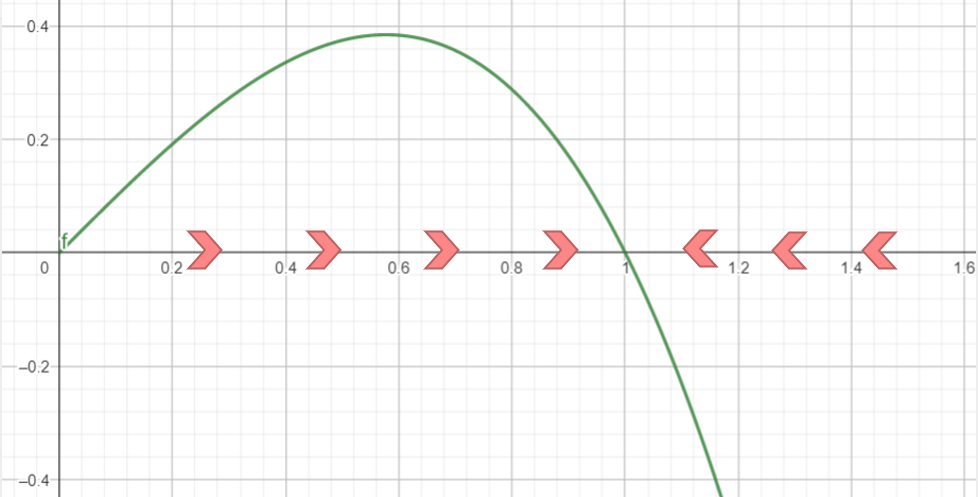
\includegraphics[width=14cm]{rej1.png}
	\caption{Plano fase de $\refeq{drsis1}$.}
\end{figure}\\

Por otro lado para $\eqref{eq: dthetasis1}$ la solución es $\theta(t)=t+\theta_0$,
donde $\theta_0=\theta(0)$.\\

Las soluciones del sistema $\eqref{eq: sis1}$ convergen a puntos sobre la
circunferencia centrada en el origen de radio $1$.\\

Resolvamos el problema de forma analítica.\\

La ecuación $\eqref{eq: drsis1}$ es separable
$$\int\frac{dr}{r(1-r^2)}=\int dt$$
integramos por fracciones parciales

$$\int\frac{dr}{r(1-r^2)}=\int\frac{dr}{r}-\int\frac{dr}{2(r+1)}-\int\frac{dr}{2(r-1)}$$
$$=\ln |r|-\frac{1}{2}\ln|r+1|-\frac{1}{2}\ln|r-1|+c_1$$

entonces
$$\ln |r|-\frac{1}{2}\ln|r+1|-\frac{1}{2}\ln|r-1|=t+c$$

desarrollamos logaritmos
$$\ln\left\lvert\frac{r^2}{r^2-1}\right\rvert=2t+c$$
$$\frac{r^2}{r^2-1}=ce^{2t}$$

$$r^2=\frac{e^{2t}}{c+e^{2t}}$$

Como $r\geq 0$
$$r=\frac{e^t}{\sqrt{c+e^{2t}}}$$
Aplicamos la condición inicial $r(0)=r_0$.\\
\\Las soluciones en coordenadas polares son:
\begin{equation}\label{eq: rsis1}
	r(t)=\frac{e^t}{\sqrt{\frac{1}{r_0^2}-1+e^{2t}}}
\end{equation}
\begin{equation}\label{eq: thetasis1}
	\theta(t)=t+\theta_0
\end{equation}
Dejaremos nuestra solución en coordenadas polares para realizar el siguiente
análisis del comportamiento asintótico.\\
\begin{enumerate}
	\item Si $r_0=1$ tenemos las ecuaciones
	      $$r(t)=1$$
	      $$\theta(t)=t+\theta_0$$
	\item Por otro lado, si $r_0>1$.
	      $$\lim_{t\to\infty}r(t)=\lim_{t\to\infty}\frac{e^t}{\sqrt{\frac{1}{r_0^2}-1+e^{2t}}}=1$$
	      $$\lim_{t\to-\infty}r(t)=\lim_{t\to-\infty}\frac{e^t}{\sqrt{\frac{1}{r_0^2}-1+e^{2t}}}=\infty$$
	\item Para $0<r_0<1$.
	      $$\lim_{t\to\infty}r(t)=\lim_{t\to\infty}\frac{e^t}{\sqrt{\frac{1}{r_0^2}-1+e^{2t}}}=1$$
	      $$\lim_{t\to-\infty}r(t)=\lim_{t\to-\infty}\frac{e^t}{\sqrt{\frac{1}{r_0^2}-1+e^{2t}}}=0$$
\end{enumerate}
Las trayectorias convergen a la circunferencia con centro en el origen
y de radio  $1$.\\

¿Qué significa que las trayectorias convergen a la circunferencia de centrada en el origen y de radio $1$?

\begin{definition} [Punto $\omega$ límite]
	Decimos que $\vec{z}\in\mathbb{R}^2$ es un punto $\omega$-límite
	de $\vec{x}_0\in\mathbb{R}^2$ si existe sucesión creciente de
	tiempos $\{t_n\}_{n\in\mathbb{N}}$
	con $t_n \to\infty$ cuando $n\to \infty$ tal que:
	$$\lim_{n\to\infty}\varphi^{t_n}(\vec{x}_0)=\vec{z}$$
\end{definition}

Regresemos las soluciones $\eqref{eq: rsis1}$ y $\eqref{eq: thetasis1}$ a
coordenadas cartesianas, con $\eqref{eq: xpolar}$ y $\eqref{eq: ypolar}$.
\begin{equation}\label{eq: xsis1}
	x(t)=\frac{e^t\cos(t+\theta_0)}{\sqrt{\frac{1}{r_0^2}-1+e^{2t}}}
\end{equation}
\begin{equation}\label{eq: ysis1}
	y(t)=\frac{e^t\sin(t+\theta_0)}{\sqrt{\frac{1}{r_0^2}-1+e^{2t}}}
\end{equation}

\begin{figure}[h]
	\centering
	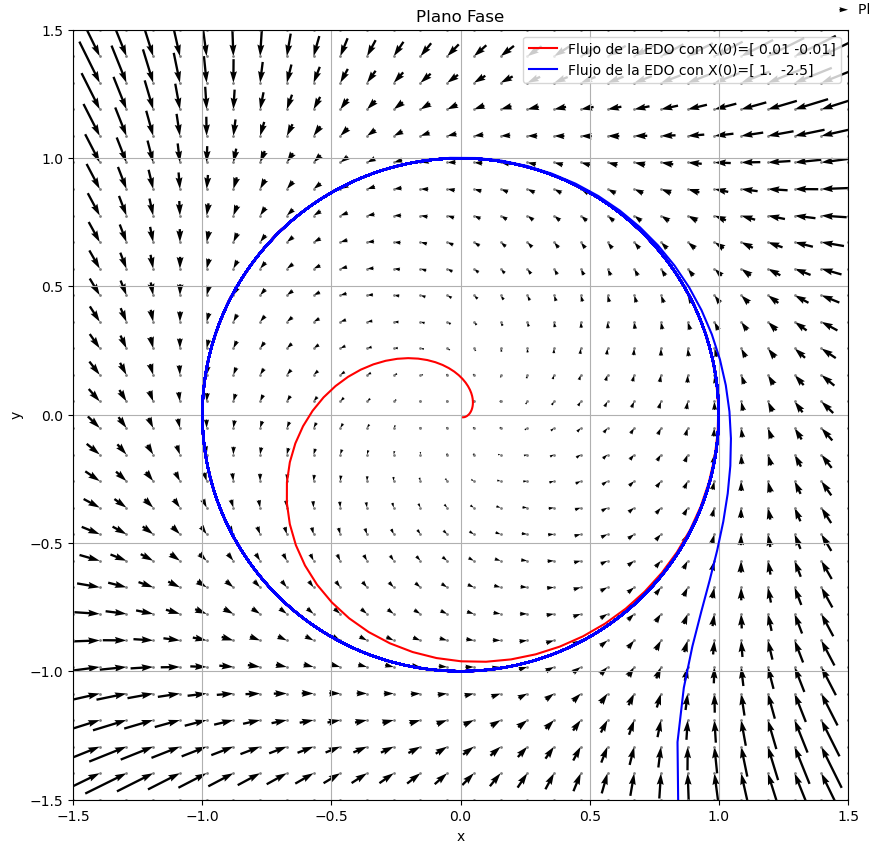
\includegraphics[width=13cm]{planofase1.png}
	\caption{Plano fase del sistema $\eqref{eq: sis1}$.}
\end{figure}

Tomemos la trayectoria en el plano fase de $\eqref{eq: sis1}$ que pasa por el punto
$(x_0,y_0)$, entonces existe $\theta_0=\arctan(\frac{y_0}{x_0})\in[0,2\pi]$.
La trayectoria que pasa por $(x_0,y_0)$ está dada por las ecuaciones $\eqref{eq: xsis1}$ y
$\eqref{eq: ysis1}$ donde $x_0=x(0)$ y $y_0=y(0)$.\\
\\Tomemos un punto en la circunferencia centrada en el origen con radio $1$,
supongamos que
en coordenadas polares tiene un álgulo $0<\alpha_0<2\pi$, veamos que es punto $\omega$ límite, para eso podemos definir
$\{t_n=2\pi n+\alpha_0-\theta_0\}_{n\in \mathbb{N}}$, entonces
$$\lim_{n\to\infty}x(t_n)=\cos(\alpha_0)$$
$$\lim_{n\to\infty}y(t_n)=\sin(\alpha_0)$$
en efecto el punto $(\cos(\alpha_0),\sin(\alpha_0))$ es un punto $\omega$ límite, esto
quiere decir que para cada punto de la circunferencia podemos encontrar
una sucesión de tiempos $\{t_n\}_{n\in \mathbb{N}}$ con $t_n\to\infty$ tal que la
trayectoria converge a ese punto de la circunferencia, es decir cualquier punto que se encuentra en la
circunferencia centrada en el origen y de radio $1$ es un punto $\omega$ límite de $(x_0,y_0)$,
entonces diremos que esta circunferencia es un conjunto $\omega$ límite de $(x_0,y_0)$, donde
el conjunto $\omega$ límite se define como

$$\omega(\vec{X}_0)=\{\vec{z}\in\mathbb{R}^2\mid\vec{z} \text{  es  } \omega\text{-límite de  } \vec{X}_0\}.$$

Además, notemos que para $\{t_n=2\pi n+\alpha_0-\theta_0\}_{n\in \mathbb{N}}$,
la sucesión $\{(x(t_n),y(t_n))\}_{n\in\mathbb{N}}$ es una sucesión
de puntos convergente tal que sus puntos son colineales sobre la recta
$L=\{(x,y)\in\mathbb{R}^2\mid y=\tan(\alpha_0)x \}$. Las intersecciones de las trayectorias
son los valores de la sucesión colineal.\\

Modifiquemos el sistema $\eqref{eq: drsis1}$, a un sistema perturbado
con $0\leq\epsilon<1$.
\begin{equation}\label{eq: drmod}
	r'=r(1-r^2)+\epsilon r\cos(\theta)
\end{equation}
Veamos si existe $r_{max}$ tal que $r'<0$ y $r_{min}$ tal que $r'>0$.\\

Reescribimos $\eqref{eq: drmod}$ como $r'=r(1-r^2+\epsilon \cos(\theta))$, como $r>0$,
entonces el signo de $r'$ depende de $1-r^2+\epsilon \cos(\theta)$.
Tenemos los siguientes casos:

\begin{enumerate}
	\item Si $1-r^2+\epsilon\cos(\theta)\leq 1-r^2+\epsilon<0$
	      entonces $\sqrt{1+\epsilon}<r_{max}$, por lo que para $r<r_{max}$ se tiene que $r'<0$.
	\item Por otro lado, si	$1-r^2+\epsilon\cos(\theta)>1-r^2-\epsilon>0$
	      entonces $\sqrt{1-\epsilon}>r_{min}$, por lo que para $r>r_{min}$ se tiene que $r'>0$.
\end{enumerate}

Las trayectorias que pasan por puntos en la circunferencia centrada
en el origen y con radio $r_{min}$
divergen del exterior de dicha circunferencia. Por otro lado,
las trayectorias que pasan por puntos en la circunferencia centrada
en el origen con radio $r_{max}$
convergen al interior del círculo.
A este segmento del plano lo llamamos región de atrapamiento.\\
\\Podemos intuir que debe existir
una curva cerrada en el interior, donde $r_{min}<r<r_{max}$, en la cual
las trayectorias convergen o alcanzan el equilibrio, de manera similar
a lo observado en el ejemplo
inicial, debido a su comportamiento. La idea de la existencia de una
curva cerrada de este tipo es lo que conocemos como ciclo límite.
\begin{figure}[h]
	\centering
	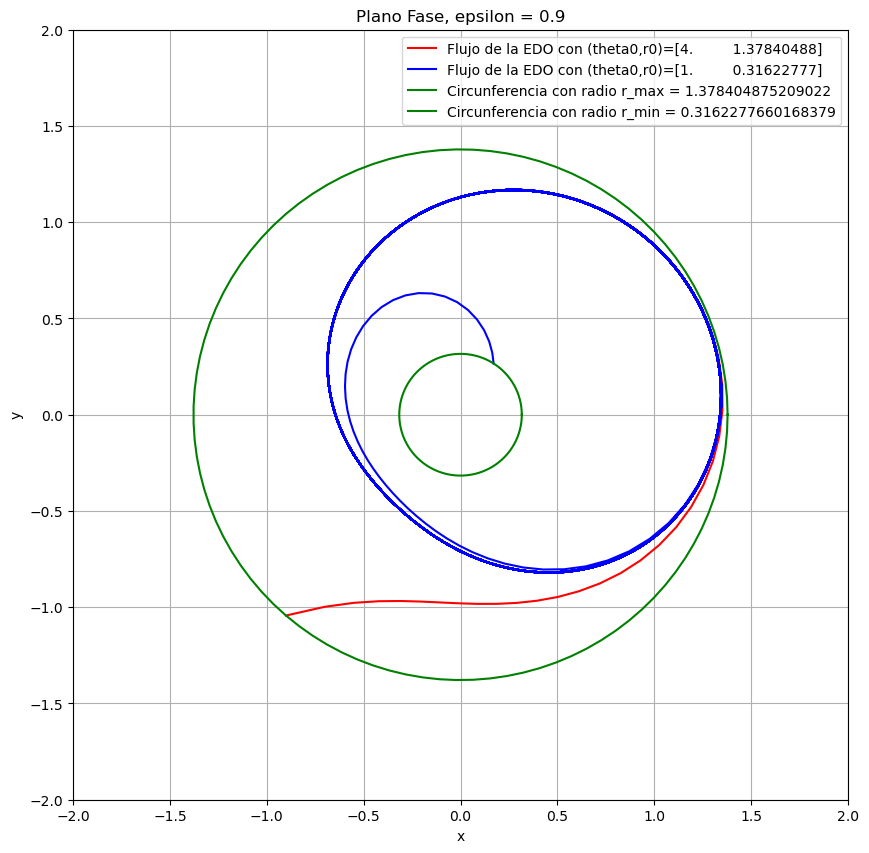
\includegraphics[width=13cm]{rminrmax.png}
	\caption{Plano fase del sistema con perturbación.}
\end{figure}

\newpage

\begin{definition}
	Definimos
	$$\varGamma_{\vec{x}}^{+}=\{\vec{y}=\varphi(t,\vec{x})\mid t>0\}$$
	$$\varGamma_{\vec{x}}^{-}=\{\vec{y}=\varphi(t,\vec{x})\mid t<0\}$$
	$$\varGamma_{\vec{x}}=\varGamma_{\vec{x}}^{+}\cup\varGamma_{\vec{x}}^{-}$$
\end{definition}

\begin{definition}
	Decimos que un conjunto $U$ es positivamente invariante si dado $\vec{x}\in U$ entonces  $\varGamma_{\vec{x}}^{+}\subset U$
\end{definition}

\begin{definition}
	Decimos que un conjunto $U$ es negativamente invariante si dado $\vec{x}\in U$ entonces  $\varGamma_{\vec{x}}^{-}\subset U$
\end{definition}

Notemos que esta sección del plano donde $r_{min}<r<r_{max}$ es positivamente invariante.
\newpage

\section{Conjuntos $\omega$ y $\alpha$ límite.}

Veamos más propiedades de los puntos y el conjunto $\omega$ límite. Comenzamos definiendo su análogo,
que estudia su comportmiento asintótico para $t\to-\infty$.\\

\begin{definition}
	Decimos que $\vec{z}\in\mathbb{R}^2$ es un punto $\alpha$-límite
	de $\vec{X}_0\in\mathbb{R}^2$ si existe sucesión decreciente de
	tiempos $\{t_n\}_{n\in\mathbb{N}}$
	con $t_n \to-\infty$ cuando $n\to \infty$ tal que:
	$$\lim_{n\to\infty}\varphi^{t_n}(\vec{X}_0)=\vec{z}$$
\end{definition}


\begin{definition}
	Definimos el conjunto $\alpha$-límite como $$\alpha(\vec{x})=\{\vec{y}\in\mathbb{R}^2\mid\vec{y}
		\text{ es } \alpha\text{-límite de }\vec{x}\}\equiv\text{Conjunto }\alpha\text{-límite}$$
	donde
	$$\vec{y}=\lim_{t_i\to-\infty}\varphi(t_i,\vec{x})$$
	con $\{t_i\}_{i=1}^{\infty}$ sucesión decreciente a $-\infty$.
\end{definition}

Algunas propiedades
\begin{itemize}
	\item $\omega(\vec{x})=\omega(\varGamma_{\vec{x}}^{+})$
	      y $\alpha(\vec{x})=\alpha(\varGamma_{\vec{x}}^{-})$.\\
	\item Si $\vec{x}*$ es equilibrio de $\vec{x}'=f(\vec{x})$ entonces:
	      $$\omega(\vec{x}*)=\alpha(\vec{x}*)=\{\vec{x}*\}$$
	\item Si $\varGamma_0$ es una órbita periódica para un sistema $\vec{X}'=f(\vec{X})$, entonces
	      $$\omega(\varGamma_0)=\alpha(\varGamma_0)=\varGamma_0$$.
\end{itemize}

\begin{lemma}
	Sea $\vec{x}\in\mathbb{R}^n$ tal que $\Gamma_{\vec{x}}^+$ esta acotada.
	Entonces:
	\begin{enumerate}
		\item $\omega(\vec{x})\neq\emptyset$
		\item $\omega(\vec{x})$ es acotado.
		\item $\omega(\vec{x})$ es cerrado.
		\item $\omega(\vec{x})$ es conexo.
	\end{enumerate}
\end{lemma}

\begin{lemma}
	Sea $\vec{x}\in\mathbb{R}^n$ con $\Gamma_{\vec{x}}^+$ acotada.
	Entonces
	$$\rho(\phi(t,\vec{x}),\omega(\vec{x}))\to0$$
	cuando $t \to \infty$.
\end{lemma}

\begin{lemma}[Invarianza]
	Sea $\Gamma_{\vec{x}}^+$ acotada. Entonces $\omega(\vec{x})$
	es invariante bajo el flujo
	$\varphi^t$, es decir, para cada $\vec{y}\in\omega(\vec{x})$ entonces
	$\varphi ^t(\vec{y})\in\omega(\vec{x})$.
\end{lemma}

\begin{lemma}
	Si $\omega(x)\neq\emptyset$ y no contiene puntos de equilibrio. Entonces contiene una órbita periódica $\varGamma_0$.
\end{lemma}

\begin{lemma}
	Si $\omega(x)$ contiene una órbita periódica $\varGamma_0$. Entonces $\omega(x)=\varGamma_0$.
\end{lemma}

\section{Teorema de Poincaré-Bendixson}

\begin{theorem}[Poincaré-Bendixson]\label{TPB}
	Sea $\vec{x}\in\mathbb{R}^2$ tal que $\varGamma_{\vec{x}}^2\subseteq D\subseteq\mathbb{R}^2$ con $D\equiv$ Cerrado y acotado,
	y conteniendo un número finito de equilirios de la EDO:
	\begin{equation}
		\begin{matrix}
			x' = f(x,y) \\
			y' = g(x,y)
		\end{matrix}
	\end{equation}
	entonces se cumple alguna de las siguientes:
	\begin{enumerate}
		\item $\omega(\vec{x})=\omega(\varGamma_{\vec{x}}^+)$ esta formado por un equilibrio.
		\item $\omega(\vec{x})$ es una órbita periódica.
		\item $\omega(\vec{x})$ está formada por equilibrios y órbitas que tienen a dichos equilibrios como puntos
		      $\alpha$ u $\omega$ límite.
	\end{enumerate}
\end{theorem}

\begin{definition}[Ciclo límite.]
	Decimos que la órbita periódica $\varGamma_0=\omega(\vec{x})$
	del caso $2$ del teorema $\ref{TPB}$ se llama
	\textbf{cliclo límite} si hay un anillo abierto que lo
	ontenga y no hay otra órbita periódica en él, es decir
	un ciclo límite es una órbita periódica aislada.

\end{definition}

\begin{definition}
	La órbita que conecta a un punto silla consigo mismo (la intersección de la variedad estable con la inestable), se le llama curva homoclínica.
\end{definition}

\begin{definition}
	La órbita que conecta dos diferentes puntos de equilibrio se le llama curva heteroclínica.

\end{definition}
\newpage

\section{Oscilador de Van der Pol}

La ecuación del oscilador de Van der Pol describe el comportamiento de ciertos sistemas oscilantes no lineales.
Su fundamento físico se basa en el concepto de amortiguamiento no lineal y autodemostración de oscilaciones.
\begin{equation}\label{eq: VP}
	x''+x+\epsilon x'(x^2-1)=0
\end{equation}
donde $\epsilon$ es un parámetro de amortiguamiento no lineal.\\
\\El término $-\epsilon(1 - x^2)x'$ representa la no linealidad del amortiguamiento en el sistema. La expresión
$(1 - x^2)$ describe cómo el amortiguamiento varía en función de la posición del oscilador. Cuando $x$ es
pequeño, este término es cercano a $1$ y el amortiguamiento es lineal. Sin embargo, a medida que $x$
aumenta, el término $(1 - x^2)$ se hace más negativo, generando un efecto de amortiguamiento no lineal que
disminuye la velocidad del oscilador.\\
\\Extendemos a un sistema de ecuaciones.
\begin{equation}\label{eq: VPsis}
	\begin{matrix}
		y'=-x-\epsilon y(x^2-1) \\
		x'=y
	\end{matrix}
\end{equation}

Los puntos de equilibrio del sistema se obtienen resolviendo \(x' = 0\) y \(y' = 0\):

\begin{equation}
    \begin{cases}
        y = 0, \\
        \epsilon (1 - x^2) y - x = 0.
    \end{cases}
\end{equation}

Sustituyendo \( y = 0 \) en la segunda ecuación, obtenemos:

\begin{equation}
    -x = 0 \implies x = 0.
\end{equation}

Por lo tanto, el único punto de equilibrio es el origen \((0, 0)\).

\subsubsection*{Matriz Jacobiana y Valores Propios}

Calculamos la matriz Jacobiana \( J \) del sistema \eqref{eq:van_der_pol_sistema}:

\begin{equation}
    J = 
    \begin{pmatrix}
        \dfrac{\partial x'}{\partial x} & \dfrac{\partial x'}{\partial y} \\
        \dfrac{\partial y'}{\partial x} & \dfrac{\partial y'}{\partial y}
    \end{pmatrix}
    =
    \begin{pmatrix}
        0 & 1 \\
        -1 - 2\epsilon x y & \epsilon (1 - x^2)
    \end{pmatrix}.
\end{equation}

Evaluando en el punto de equilibrio \((0, 0)\):

\begin{equation}
    J|_{(0,0)} = 
    \begin{pmatrix}
        0 & 1 \\
        -1 & \epsilon
    \end{pmatrix}.
\end{equation}

Obtenemos los valores propios \(\lambda\) resolviendo el determinante característico:

\begin{equation}
    \det(J - \lambda I) = 0,
\end{equation}

es decir,

\begin{equation}
    \left| \begin{array}{cc}
        -\lambda & 1 \\
        -1 & \epsilon - \lambda
    \end{array} \right| = 0.
\end{equation}

Calculamos el determinante:

\begin{equation}
    (-\lambda)(\epsilon - \lambda) - (-1)(1) = \lambda^2 - \epsilon \lambda + 1 = 0.
\end{equation}

Resolviendo la ecuación cuadrática:

\begin{equation}
    \lambda = \frac{\epsilon \pm \sqrt{\epsilon^2 - 4}}{2}.
\end{equation}

Para \(\epsilon > 0\), si \(\epsilon^2 - 4 > 0\) (es decir, \(\epsilon > 2\)), los valores propios son reales y positivos, lo que indica que el punto de equilibrio es un \textbf{nodo inestable}. Si \(0 < \epsilon < 2\), los valores propios son complejos con parte real positiva, lo que implica que el origen es un \textbf{foco inestable}.

\subsection*{Aplicación del Teorema de Poincaré-Bendixson}

Para demostrar la existencia de un ciclo límite, utilizamos el \textbf{teorema de Poincaré-Bendixson}, que establece que si un conjunto compacto, invariante y sin puntos de equilibrio en su interior existe para un sistema planar, entonces el sistema tiene una órbita periódica dentro de ese conjunto.

\subsubsection{Construcción de una Región Acotada Invariante}

Definimos una función de Lyapunov candidata:

\begin{equation}
    V(x, y) = \dfrac{1}{2} \left( x^2 + y^2 \right).
\end{equation}

Calculamos la derivada total de \( V \) respecto al tiempo:

\begin{equation}
    \dot{V} = x \dot{x} + y \dot{y} = x y + y \left( \mu (1 - x^2) y - x \right) = y^2 \left( \mu (1 - x^2) \right).
\end{equation}

Analizamos el signo de \( \dot{V} \):

\begin{itemize}
    \item Para \( |x| > 1 \), se tiene \( x^2 > 1 \), por lo que \( 1 - x^2 < 0 \) y entonces:

    \begin{equation}
        \dot{V} = y^2 \mu (1 - x^2) < 0.
    \end{equation}

    Esto indica que en la región donde \( |x| > 1 \), la energía total \( V \) decrece, y las trayectorias se dirigen hacia el interior de esta región.

    \item Para \( |x| < 1 \), se tiene \( 1 - x^2 > 0 \), y por lo tanto \( \dot{V} > 0 \), indicando que en esta región la energía total \( V \) aumenta, y las trayectorias se alejan del origen.
\end{itemize}

Concluimos que las trayectorias que empiezan fuera del círculo \( x^2 + y^2 = R^2 \) con \( R > 1 \) eventualmente entran en esta región y permanecen en un conjunto compacto y acotado.

Dado que:

\begin{enumerate}
    \item El sistema es plano y continuo.
    \item Existe una región compacta e invariante (por la función de Lyapunov) sin puntos de equilibrio distintos del origen.
    \item El origen es un punto de equilibrio inestable.
\end{enumerate}

Aplicando el teorema de Poincaré-Bendixson, concluimos que existe al menos una órbita periódica (ciclo límite) en la región acotada definida.

\section{Ecuación de Rayleigh}
La ecuación de Rayleigh con amortiguamiento no lineal, se utiliza
para estudiar oscilaciones no lineales en sistemas mecánicos y se encuentra en
diversos campos como la mecánica estructural y la dinámica de sistemas físicos.

$$x''+\epsilon(x'^2-1)x'+x=0$$

El parámetro $\epsilon$ es un coeficiente que controla la influencia del término no lineal en el amortiguamiento.
El término $\epsilon(x'^2 - 1)x'$ es el término no lineal en el amortiguamiento. Mientras que en el amortiguamiento
lineal la fuerza de amortiguamiento es proporcional a la velocidad, en este caso el amortiguamiento depende de
la velocidad al cuadrado y se modifica por el término $(x'^2 - 1)$. Esto introduce un comportamiento no lineal en e
l sistema y puede dar lugar a fenómenos como la autoexcitación y la respuesta no armónica.
Extendemos a un sistema de ecuaciones.

\begin{equation}\label{eq: Rayleigh}
	\begin{matrix}
		y'=-\epsilon(y^2-1)y-x \\
		x'=y
	\end{matrix}
\end{equation}


Los puntos de equilibrio se encuentran resolviendo \(\dot{x} = 0\) y \(\dot{y} = 0\):

\begin{equation}
    \begin{cases}
        y = 0, \\
        \epsilon \left(1 - y^2\right) y - x = 0.
    \end{cases}
\end{equation}

Sustituyendo \( y = 0 \) en la segunda ecuación, obtenemos:

\begin{equation}
    - x = 0 \implies x = 0.
\end{equation}

Por lo tanto, el único punto de equilibrio es el origen \((0, 0)\).

\subsubsection{Matriz Jacobiana y Valores Propios}

Calculamos la matriz Jacobiana \( J \) del sistema \eqref{eq:rayleigh_sistema}:

\begin{equation}
    J =
    \begin{pmatrix}
        \dfrac{\partial \dot{x}}{\partial x} & \dfrac{\partial \dot{x}}{\partial y} \\
        \dfrac{\partial \dot{y}}{\partial x} & \dfrac{\partial \dot{y}}{\partial y}
    \end{pmatrix}
    =
    \begin{pmatrix}
        0 & 1 \\
        -1 & \epsilon \left(1 - 3 y^2\right)
    \end{pmatrix}.
\end{equation}

Evaluamos en el punto de equilibrio \((0, 0)\):

\begin{equation}
    J|_{(0,0)} =
    \begin{pmatrix}
        0 & 1 \\
        -1 & \epsilon
    \end{pmatrix}.
\end{equation}

Los valores propios \(\lambda\) se obtienen resolviendo:

\begin{equation}
    \det(J - \lambda I) = \left| \begin{array}{cc}
        -\lambda & 1 \\
        -1 & \epsilon - \lambda
    \end{array} \right| = 0.
\end{equation}

Calculamos el determinante:

\begin{equation}
    (-\lambda)(\epsilon - \lambda) - (-1)(1) = \lambda^2 - \epsilon \lambda + 1 = 0.
\end{equation}

Resolviendo la ecuación cuadrática:

\begin{equation}
    \lambda = \dfrac{\epsilon \pm \sqrt{\epsilon^2 - 4}}{2}.
\end{equation}

\begin{itemize}
    \item Si \(\epsilon^2 - 4 > 0\) (es decir, \(\epsilon > 2\)), los valores propios son reales y de signos opuestos si \(\epsilon > 0\), lo que indica un \textbf{silla de montar} en el origen.
    \item Si \(\epsilon^2 - 4 < 0\) (es decir, \(0 < \epsilon < 2\)), los valores propios son complejos conjugados con parte real positiva, ya que \(\epsilon > 0\). Esto implica que el origen es un \textbf{foco inestable}.
\end{itemize}

\subsection*{Aplicación del Teorema de Poincaré-Bendixson}

Para demostrar la existencia de un ciclo límite, aplicaremos el teorema de Poincaré-Bendixson, mostrando que las trayectorias están confinadas en una región acotada y que no hay otros puntos de equilibrio en esa región aparte del origen.

\subsubsection{Construcción de una Región Acotada Invariante}

Consideramos la siguiente función de Lyapunov candidata:

\begin{equation}
    V(x, y) = \dfrac{1}{2} y^2 + \dfrac{1}{2} x^2.
\end{equation}

Calculamos su derivada temporal:

\begin{align}
    \dot{V} &= y \dot{y} + x \dot{x} \\
    &= y \left[ \epsilon \left(1 - y^2\right) y - x \right] + x y \\
    &= y \left[ \epsilon \left(1 - y^2\right) y - x \right] + x y \\
    &= \epsilon y^2 \left(1 - y^2\right) - y x + x y \\
    &= \epsilon y^2 \left(1 - y^2\right).
\end{align}

Analizamos el signo de \(\dot{V}\):

\begin{itemize}
    \item Para \( |y| > 1 \), se tiene \( y^2 > 1 \), entonces \( 1 - y^2 < 0 \) y por lo tanto:

    \begin{equation}
        \dot{V} = \epsilon y^2 (1 - y^2) < 0.
    \end{equation}

    Esto indica que las trayectorias se dirigen hacia la región donde \( |y| \leq 1 \).

    \item Para \( |y| < 1 \), se tiene \( 1 - y^2 > 0 \), y por lo tanto:

    \begin{equation}
        \dot{V} = \epsilon y^2 (1 - y^2) \geq 0.
    \end{equation}

    En esta región, la energía \( V \) no decrece, pero debido a la inestabilidad en el origen, las trayectorias tienden a alejarse del punto de equilibrio.
\end{itemize}

Observamos que:

\begin{enumerate}
    \item Las trayectorias que empiezan fuera de la región \( |y| \leq 1 \) eventualmente entran en esta región y quedan confinadas en un conjunto compacto debido a la disminución de \( V \).

    \item No hay otros puntos de equilibrio distintos del origen en esta región.

    \item El origen es inestable (foco inestable o silla de montar dependiendo del valor de \(\epsilon\)).
\end{enumerate}

Por el \textbf{teorema de Poincaré-Bendixson}, existe al menos un ciclo límite en esta región acotada.

\section{Sistemas Lienard}

Los sistemas Lienard son ecuaciones diferenciales de la forma:
\begin{equation}\label{eq: lienard}
	x''+f(x)x'+g(x)=0
\end{equation}
Para extender esta ecuacipon diferencial a un sistema de ecuaciones diferenciales. Primero definimos
$$F(x)=\int_0^xf(s)ds$$
entonces haciendo el cambio de variable $y=x'+F(x)$, obtenemos el sistema:
\begin{equation}\label{eq: lienardsystem}
	\begin{matrix}
		x'=y-F(x) \\
		y'=-g(x)
	\end{matrix}
\end{equation}
Vamos a enunciar el siguiente importante teorema.
\begin{theorem}[Lienard]
	Si $F(x)$ y $g(x)$ del sistema $\eqref{eq: lienardsystem}$ satisfacen las siguientes hipótesis:
	\begin{enumerate}
		\item $F,g\in C^1$.
		\item $F$ y $g$ son funciones impares.
		\item $xg(x)>0$ para todo $x\neq 0$.
		\item $F'(0)<0$
		\item $F$ tiene ceros sólo en $x=0$ o en $x=\pm a$.
		\item $F$ es monótona creciente en $(a,\infty)$ y $\lim_{x\to\infty}F(x)=\infty$
	\end{enumerate}
	entonces el sistema $\eqref{eq: lienardsystem}$ tiene un único ciclo límite y es estable.
\end{theorem}
Veamos que el sistema de ecuaciones asociado al Oscilador de Van der Pol es un sistema Lienard.
$$x''+\epsilon(x^2-1)x'+x=0$$
Definimos
$$F(x)=\int_0^x\epsilon(s^2-1)ds$$
$$=\epsilon[\frac{1}{3}s^3-s]| _0^x=\epsilon[\frac{1}{3}x^3-x]$$
Tenemos $F(x)=\frac{\epsilon}{3}[x^3-3x]$ y $g(x)=x$.\\
\\Podemos extender el oscilador de Van der Pol al sistema de ecuaciones:
$$
	\begin{matrix}
		x'=y-\frac{\epsilon}{3}[x^3-3x] \\
		y'=-x
	\end{matrix}
$$
Veamos si $F$ y $g$ satisfacen las hipótesis del teorema de Lienard
\begin{enumerate}
	\item En efecto $F,g\inC^1$.
	\item Notemos que las funciones son impares
	      $$F(-x)=\frac{\epsilon}{3}[(-x)^3-3(-x)]=\frac{\epsilon}{3}[-x^3+3x]=-\frac{\epsilon}{3}[x^3-3x]=-F(x)$$
	      $$g(-x)=-x=-g(x)$$.
	\item $xg(x)=x(x)=x^2>0$ para todo $x\neq 0$.
	\item $F'(0)=\epsilon(0^2-1)=-\epsilon<0$
	\item $F(x)=\frac{\epsilon}{3}[x^3-3x]=0$ entonces $F$ tiene raíces en $x=0$ y  $x=\pm \sqrt{3}$
	\item Si $y>x>\sqrt{3}$, entonces $y^3-3y>x^3-3x$, por lo que $F$ es monótona creciente. Además
	      por ser una función polinomial se tiene que
	      $$\lim_{x\to\infty}F(x)=\infty.$$
\end{enumerate}
Por lo tanto, por el teorema de Lienard el oscilador de Van der Pol tiene un único ciclo límite y es estable.
Esto ya lo comprobamos anteriormente, pero este teorema nos garantiza que es el único ciclo límite.

\chapter{Teoría de promediación}

Como vimos determinar la existencia y propiedades cualitativas y cuantitativas
de los ciclos límite en sistemas no lineales no es tarea fácil. En muchos
casos los métodos analíticos fallan o se vuelve sumamente complejo y los
métodos numéricos pueden ser ineficientes o inexactos. \\

El Método de Promediación es una herramienta poderosa y efectiva,
parte de la teoría de perturbaciones y nos ayuda a simplificar el análisis
de sistemas no lineales  transformando las ecuaciones originales en un sistema
más manejable. La premisa fundamental es que, bajo ciertas condiciones, el
comportamiento promedio del sistema a lo largo del tiempo puede revelar
la existencia y la estructura de los ciclos límite.\\

La aplicación del Método de Premediación para verificar la existencia de
ciclos límite en sistemas no lineales no solo proporciona una técnica
analítica robusta sino que también ofrece una perspectiva más profunda
del comportamiento oscilatorio inherente en dichos sistemas. Este enfoque
no solo permite simplificar las ecuaciones diferenciales originales, sino
también captar la esencia del comportamiento dinámico del sistema,
facilitando así la identificación y caracterización de ciclos límite.\\

Definiendo el promedio local de una función y algunas de sus propiedades.

\section{Método de promediación}

\begin{definition}
	Sea $f:\mathbb{R}\times\mathbb{R}^p\to\mathbb{R}^n$ continua y $T>0$.
	Definimos:
	$$
		f_T(t,x)=\frac{1}{T}\int_{0}^{T}f(t+\tau,x)d\tau
	$$
	como el promedio local de $f$.
\end{definition}
\\
La función $f_T(t,x)$ calcula el valor promedio de la función $f(t,x)$ 
respecto a la variable $t$ en el intervalo $[t,t+T]$, visto de otro 
modo, calcula el comportamiento promedio futuro del tiempo $t$ a tiempo $t+T$.

\begin{proposition}
	Sea $f:\mathbb{R}\times\mathbb{R}^p\to\mathbb{R}^n$ continua y de periodo $T$ en $t$, entonces
	$$
		f_T(t,x)=f_0(x)
	$$
\end{proposition}
\\
Si la función a promediar es de Lipschitz entonces la diferencia entre ambas
funciones está acotada, esto quiere decri que el mapeo del promedio local de 
la función no se aleja demasiado de la función original, solo lo simplifica 
y guarda el comportamiento promedio de la función.
\begin{proposition}
	Si $\phi:\mathbb{R}\to\mathbb{R}$ es de Lipschitz en $\mathbb{R}$ con constante de Lipschitz $\lambda$ entonces
	$$
		\abs{\phi(x)-\phi_T(x)}\leq\frac{\lambda T}{2}
	$$
	i.e. $\phi(t)$ es $o(T)$ con respecto a $\phi_T(x)$.
\end{proposition}
\\
\begin{example}
	Consideremos la función $\phi(t)=\sqrt{t^2+1}$, esta función es de Lipschitz
	con constante $\lambda=1$, calculamos su promedio local con $T=0.5$

	$$\phi_T(t)=\frac{1}{2T}(((T + t)\sqrt{1 + (T + t)^2} + \sinh^{-1}(T + t)) - (t\sqrt{1 + t^2} + \sinh^{-1}(t)))$$

	graficamos ambas funciones.

	\begin{figure}[h]
		\centering
		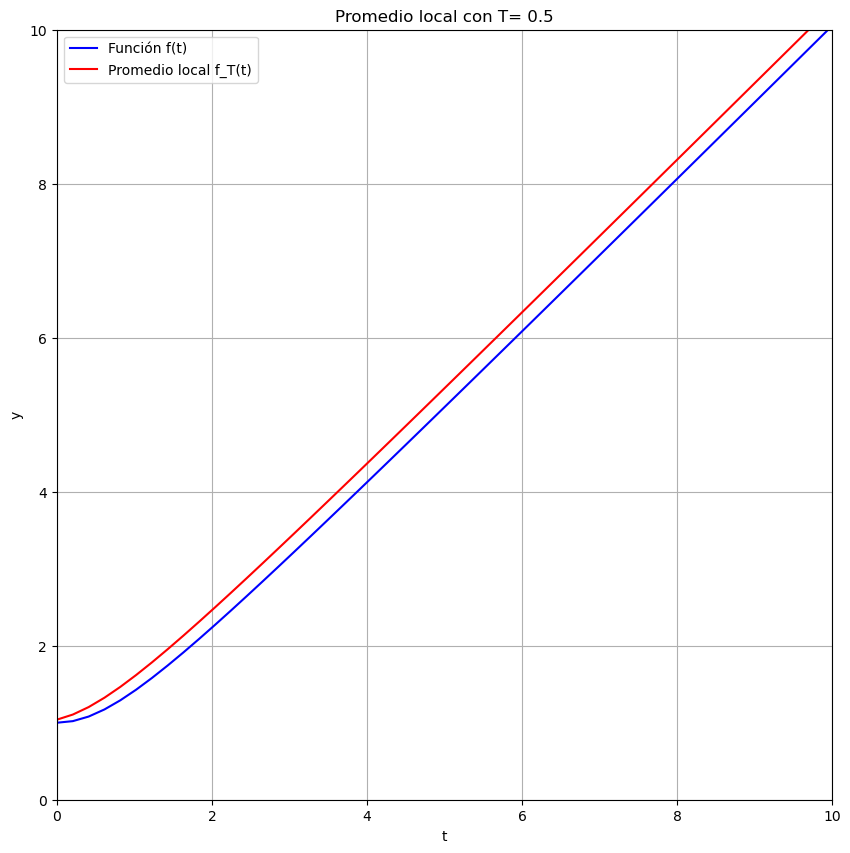
\includegraphics[width=10cm]{fl.png}
		\caption{Función vs  función promediada.}
	\end{figure}

	la diferencia esta acotada por $M=\frac{\lambda T}{2}=\frac{0.5}{2}=0.25$. En este caso en la
	gráfica se puede observar que la diferencia converge a la cota $M$.

	\begin{figure}[h]
		\centering
		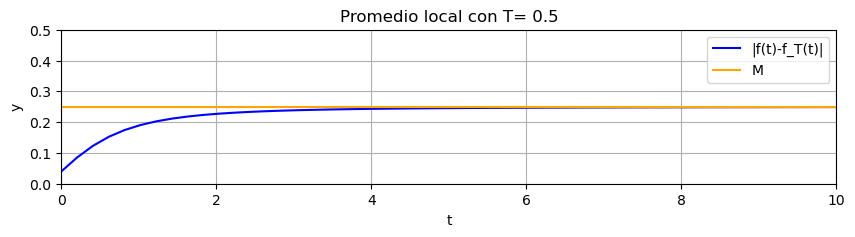
\includegraphics[width=13cm]{d.png}
		\caption{Diferencia de la Función con la función promediada.}
	\end{figure}

\end{example}

\newpage

este comportamiento asintótico no necesariamente ocurre siempre, un ejemplo es la función $\sin(x)$. 

\begin{lemma}
	Consideremos la EDO
	$$
		x'=\epsilon f(t,x)
	$$
	con $x(0)=x_0$, donde $f$ es de Lipschitz en $x\in D\subseteq\mathbb{R}^n$
	y $f$ continua en $t\in[0,t]$.\\
	Sea $M=\sup_{x\in D} \sup_{0\leq\epsilon t\leqL} \abs{f(t,x)}<+\infty$
	\\Si $\phi(t)=\int_{0}^{t}f(\tau,x(\tau))d\tau$ con $x$ solución de la EDO.
	\\Entonces:
	$$
		\abs{\phi_T(t)-\int_{0}^{t}f_T(\tau,x(\tau))d\tau}\leq\frac{1}{2}(1+\lambda L)MT
	$$
	para $o(\frac{1}{\epsilon})=t$, donde $\lambda\equiv cte$ de Lipschitz.
	\\i.e. $\phi_T(t)=\int_{0}^{t}f_T(\tau,x(\tau))d\tau+o(T)$
\end{lemma}

\begin{lemma}
	Consideremos el problema de valor inicial
	$$
		x'=\epsilon f(t,x)
	$$
	$x(0)=x_0$, con $f$ Lipschitz en $x\in D\subseteq\mathbb{R}^n$ y continua
	en $t\in[0,t]$. \\
	Si $y$ es solución de $y'=\epsilon f_T(t,y)$, $y(0)=x_0$, entonces
	$$
		x(t)-y(t)=o(\epsilon T)
	$$
	p.t. $t=o(\frac{1}{\epsilon})$
\end{lemma}

\begin{theorem}
	Consideremos $x'=\epsilon f(t,x)$, $x(t_0)=x_0$ y $y'=f^0(y)$, $y(t_0)=x_0$,
	donde $x_0,x,y\in D\subseteq\mathbb{R}^n$ y $\epsilon\in[0,\epsilon_0]$.\\

	Satisfaciendo:
	\begin{enumerate}
		\item $\bar{f}(t,x)$ es $T$ periódica con promedio $f^0(x)$.
		\item $f$ es continua en $t$ y Lipschitz en $x\in D$.
		\item $y(t)$ permanece en el interior de $D$ para todo $t=O(\frac{1}{\epsilon})$.
	\end{enumerate}
	Entonces
	$$x(t)-y(t)=O(\delta(\epsilon))$$
	para todo $t=o(\frac{1}{\epsilon})$ con $\delta=\delta(\epsilon)$ función de orden.
\end{theorem}

\section{Oscilador de Van der Pol}
De nuevo vamos a trabajar e Oscilador de Van der Pol pero ahora vamos a implementar la teoría de promediación para demostrar la existencia de ciclos límite.\\

Sea el sistema de ecuaciones

\begin{equation}\label{eq: VPsis}
	\begin{matrix}
		y'=-x-\epsilon y(x^2-1) \\
		x'=y
	\end{matrix}
\end{equation}

Haremos el cambio de coordenadas a polares.
Sustituimos en $\eqref{eq: dxpolar}$ y $\eqref{eq: dypolar}$ en $\eqref{eq: VPsis}$
$$r\cos(\theta)\theta'+r'\sin(\theta)=-r\cos(\theta)-\epsilon r\sin(\theta)(r^2\cos^2(\theta)-1)$$
$$-r\sin(\theta)\theta'+r'\cos(\theta)=r\sin(theta)$$
entonces
\begin{equation}\label{eq: VPdr}
	r'=-\epsilon r\sin^2(\theta)(r^2\cos^2(\theta)-1)
\end{equation}
\begin{equation}\label{eq: VPdtheta}
	\theta'=-1-\epsilon r\sin(\theta)\cos(\theta)(r^2\cos(\theta^2)-1)
\end{equation}
Definimos para $\eqref{eq: VPdr}$ el promedio
\begin{equation}\label{eq: drbar}
	\bar{r}'=\bar{f}(\bar{r},\epsilon)
\end{equation}
donde
$$\bar{f}(\bar{r},\epsilon)=\frac{1}{2\pi}\int\limits_0^{2\pi}r'd\theta$$
Calculamos esta integral
$$\bar{f}(\bar{r},\epsilon)=\frac{1}{2\pi}\int\limits_0^{2\pi}-\epsilon r\sin^2(\theta)(r^2\cos^2(\theta)-1)d\theta$$
$$=\frac{1}{2\pi}[-\epsilon r^3\int\limits_0^{2\pi}\sin^2(\theta)\cos^2(\theta)d\theta+\epsilon r\int\limits_0^{2\pi}\sin^2(\theta)d\theta]$$
$$=\frac{1}{2\pi}[-\epsilon r^3[\frac{1}{32}(4\theta-\sin(4\theta))]_0^{2\pi}+\epsilon r[\frac{1}{2}(\theta-\sin(\theta)\cos(\theta))]_0^{2\pi}]$$
$$=\frac{1}{2\pi}[\frac{-\epsilon r^3}{32}(8\pi)+\frac{\epsilon r}{2}(2\pi)]=\frac{1}{2\pi}[\frac{-\epsilon r^3}{4}\pi+\epsilon r\pi].$$
Entonces
$$\bar{f}(\bar{r},\epsilon)=\frac{\epsilon r}{2}-\frac{\epsilon r^3}{8}$$
Pormediamos $\theta$
$$\bar{\theta}=2\pi t$$
Vamos a analizar $\eqref{eq: drbar}$
\begin{equation}\label{eq: drvander}
	\bar{r}'=\frac{\epsilon}{8}r(4-r^2)
\end{equation}
\begin{figure}[h]
	\centering
	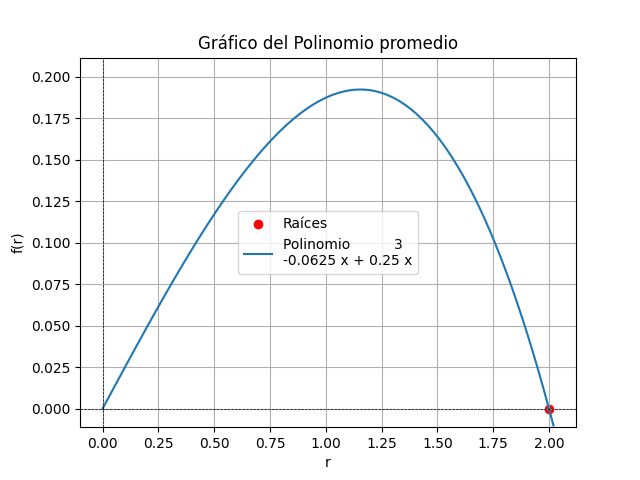
\includegraphics[width=14cm]{graficavanderpol.png}
	\caption{Plano fase de $\eqref{eq: drvander}$.}
\end{figure}
Las soluciones de equilibrio son $r=0$ y $r=2$.
\begin{enumerate}
	\item Si $0<r<2$, entonces $r'>0$, por lo que $0$ es un punto fuente o repulsivo.
	\item Si $r>2$, entonces $r'<0$, entonces $r=2$ es sumidero o atractor.
\end{enumerate}\\

\begin{figure}[h]
	\centering
	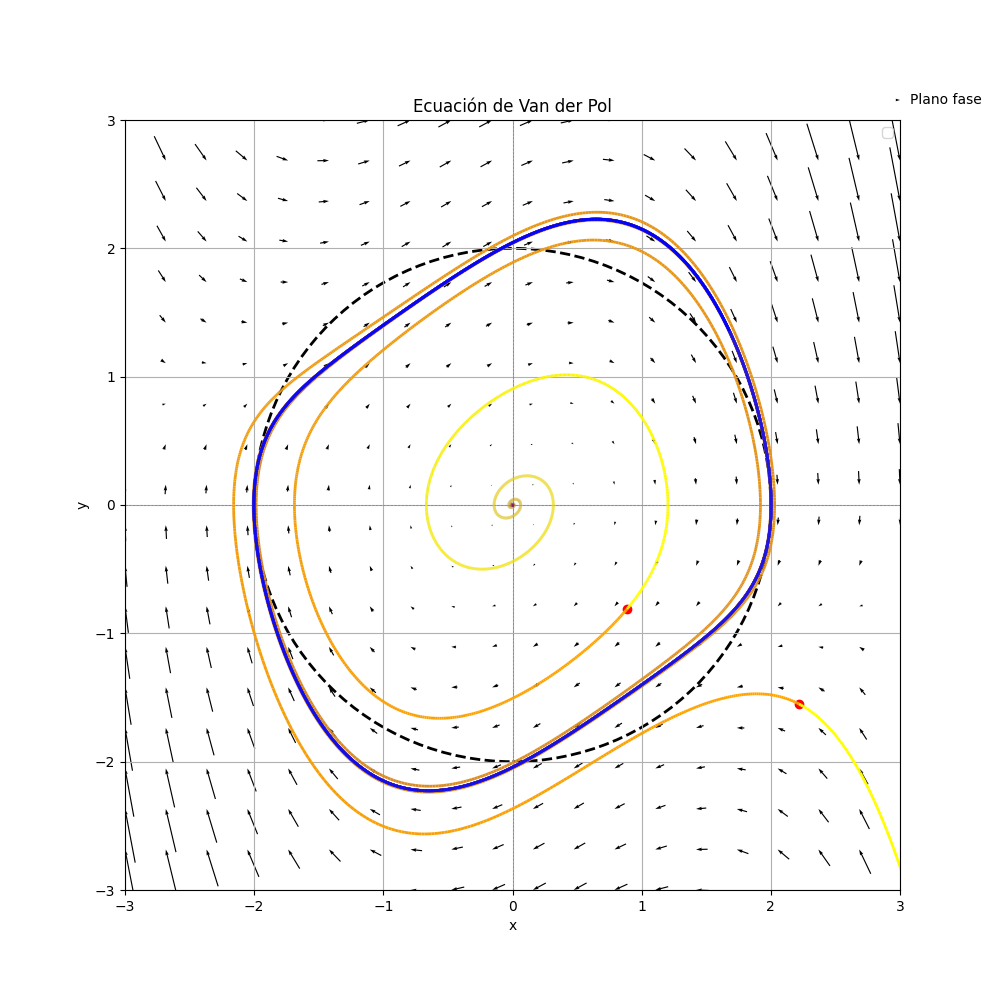
\includegraphics[width=11cm]{vanderpol.png}
	\caption{Plano fase. Dibujado en https://aeb019.hosted.uark.edu/pplane.html}
\end{figure}
\\Esto quiere decir que entre dos circunferencias de radios $0<r_{min}<2$ y $2<r_{max}$
existe al menos una curva cerrada a la cual las curvas convergen.

\newpage

\section{Ecuación de Rayleigh}

Vamos a implementar en la ecuación de Rayleigh la teoría de promediación para demostrar la existencia de ciclos límite.

\begin{equation}\label{eq: Rayleigh}
	\begin{matrix}
		y'=-\epsilon(y^2-1)y-x \\
		x'=y
	\end{matrix}
\end{equation}

Haremos el cambio de coordenadas a polares.
$$r\cos(\theta)\theta'+r'\sin(\theta)=-\epsilon (r^2\sin^2(\theta)-1)r\sin(\theta)-\omega^2r\cos(\theta) $$
$$-r\sin(\theta)\theta'+r'\cos(\theta)=r\sin(\theta)$$
Obtenemos la ecuación.
\begin{equation}\label{eq: Rayleighpolar}
	r'=\epsilon(1-r^2\sin^2(\theta))r\sin^2(\theta)+r\sin(\theta)\cos(\theta)(1-\omega^2)
\end{equation}
Definimos para $\eqref{eq: Rayleighpolar}$ el promedio
$$\bar{r}=\bar{f}(\bar{r},\epsilon)=\frac{1}{2\pi}\int\limits_0^{2\pi}r'd\theta$$
Calculamos esta integral
$$\bar{f}(\bar{r},\epsilon)=\frac{1}{2\pi}\int\limits_0^{2\pi}[\epsilon(1-r^2\sin^2(\theta))r\sin^2(\theta)+r\sin(\theta)\cos(\theta)(1-\omega^2)]d\theta$$
$$=\frac{1}{2\pi}\epsilon r\int\limits_0^{2\pi}\sin^2(\theta)d\theta-\frac{1}{2\pi}\epsilon r^3\int\limits_0^{2\pi}\sin^4(\theta)d\theta+\frac{1}{2\pi}r(1-\omega^2)\int\limits_0^{2\pi}\cos(\theta)\sin(\theta)d\theta$$
$$=\frac{1}{2\pi}\epsilon r[\frac{1}{2}(\theta-\sin(\theta)\cos(\theta))]\Big|_2^{2\pi}-\frac{1}{2\pi}\epsilon r^3[\frac{1}{32}(-8\sin(2\theta)+\sin(4\theta)+12\theta)]\Big|_0^{2\pi}+$$
$$\frac{1}{2\pi}r(1-\omega^2)[\cos^2(\theta)]\Big|_0^{2\pi}]=\frac{1}{2\pi}\epsilon r\pi-\frac{1}{2\pi}\epsilon r^3\frac{3}{4}\pi$$
$$=\frac{\epsilon r}{8}(4-3r^2)$$
Entonces tenemos el sistema
$$\bar{r}'=\frac{\epsilon r}{8}(4-3r^2)$$
$$\bar{\theta}'=2\pi t$$
Las soluciones de equilibrio son $r=0$ y $r=\frac{2}{3}\sqrt{3}$
\begin{figure}[h]
	\centering
	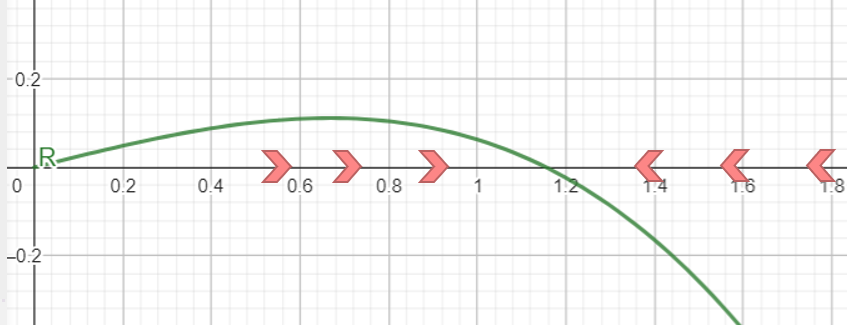
\includegraphics[width=9cm]{graficarayleigh.png}
	\caption{Plano fase.Dibujado en https://aeb019.hosted.uark.edu/pplane.html}
\end{figure}
\begin{figure}[h]
	\centering
	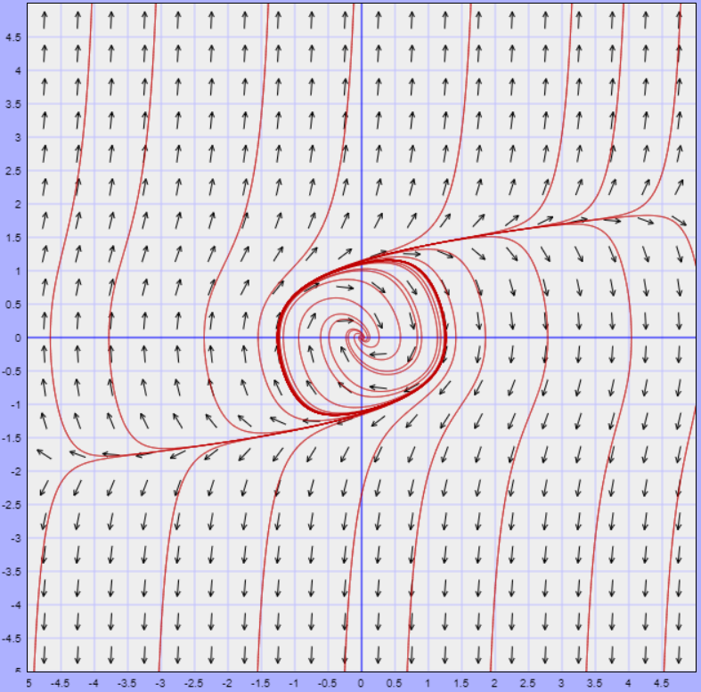
\includegraphics[width=11cm]{planorayleigh.png}
	\caption{Plano fase.Dibujado en https://aeb019.hosted.uark.edu/pplane.html}
\end{figure}

\newpage




\section{Van der Pol y Rayleigh}
Ahora vamos a analizar la EDO
\begin{equation}\label{eq: vdpr}
	x''+\epsilon(x'^2-1)x'+\eta(x^2-1)x'+x=0
\end{equation}
Extendemos esta ecuación a un sistema de ecuaciones haciendo el
cambio de variable usual $y=x'$. Obetenemos lo siguiente:
\begin{equation}\label{eq: vpdrsis}
	\begin{matrix}
		y'=-\epsilon(y^2-1)x'-\eta(x^2-1)y-x \\
		x'=y
	\end{matrix}
\end{equation}
Hamos un cambio de coordenadas a polares. Sustituimos $\eqref{eq: dxpolar}$ y
$\eqref{eq: dypolar}$ en nuestro sistema, obtenemos:
$$r'\sin(\theta)+\theta'r\cos(\theta)=-\epsilon(r^2\sin^2(\theta)-1)r\sin(\theta)-\eta(r^2\cos^2(\theta)-1)r\sin(\theta)-r\cos(\theta)$$
$$r'\cos(\theta)-\theta'r\sin(\theta)=r\sin(\theta)$$
Calculamos $r'$ y $\theta'$
\begin{equation}\label{eq: drvdpr}
	r'=-[\epsilon(r^2\sin^2(\theta)-1)+\eta(r^2\cos^2(\theta)-1)]r\sin^2(\theta)
\end{equation}
$$\theta'=-[\epsilon(r^2\sin^2(\theta)-1)+\eta(r^2\cos^2(\theta)-1)]\cos(\theta)\sin(\theta)-r$$
Vamos a promediar $r'$, calculamos $\bar{r}'$:
$$\bar{r}'=\frac{1}{2\pi}\int_0^{2\pi}-[\epsilon(r^2\sin^2(\theta)-1)+\eta(r^2\cos^2(\theta)-1)]r\sin^2(\theta)d\theta$$
$$=-\frac{r^3}{8}(3\epsilon+\eta)+\frac{r}{2}(\epsilon+\eta)$$
Calculamos las raíces no negativas de $\bar{r}'=-r^3(\frac{3\epsilon+\eta}{8})+r(\frac{\epsilon+\eta}{2})$, estas son
$r_1=0$ y $r_2=2\sqrt{\frac{\epsilon+\eta}{3\epsilon+\eta}}$.\\
\\Para los valores de $\epsilon=0.5$ y $\eta=0.4$ el valor de el atractor es $r_2=1.3764\dots$, podemos ver en la imagen que en efecto
existe un ciclo límite aproximado a la circunferencia de radio $r_2$.

\begin{figure}[h]
	\centering
	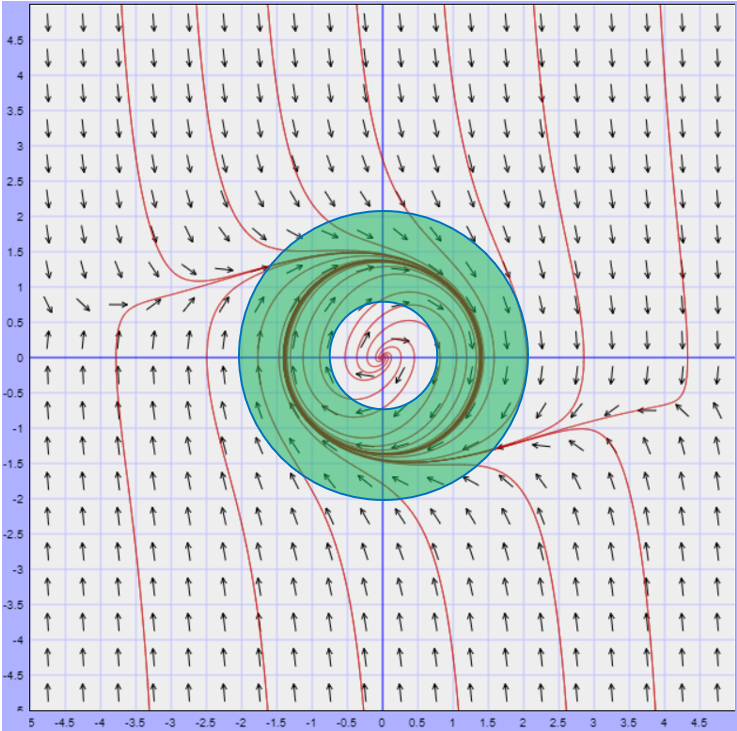
\includegraphics[width=9cm]{VDP-R.png}
	\caption{Plano fase.Dibujado en https://aeb019.hosted.uark.edu/pplane.html}
\end{figure}

\newpage








\end{document}
